%%%%%%%%%%%%%%%%%%%%%%%%%%%%%%%%%%%%%%%%%
% Beamer Presentation
% LaTeX Template
% Version 2.0 (March 8, 2022)
%
% This template originates from:
% https://www.LaTeXTemplates.com
%
% Author:
% Vel (vel@latextemplates.com)
%
% License:
% CC BY-NC-SA 4.0 (https://creativecommons.org/licenses/by-nc-sa/4.0/)
%
%%%%%%%%%%%%%%%%%%%%%%%%%%%%%%%%%%%%%%%%%

%----------------------------------------------------------------------------------------
%	PACKAGES AND OTHER DOCUMENT CONFIGURATIONS
%----------------------------------------------------------------------------------------

\documentclass[
	11pt, % Set the default font size, options include: 8pt, 9pt, 10pt, 11pt, 12pt, 14pt, 17pt, 20pt
	%t, % Uncomment to vertically align all slide content to the top of the slide, rather than the default centered
	%aspectratio=169, % Uncomment to set the aspect ratio to a 16:9 ratio which matches the aspect ratio of 1080p and 4K screens and projectors
]{beamer}

\graphicspath{{img/}{./}} % Specifies where to look for included images (trailing slash required)

\usepackage{booktabs} % Allows the use of \toprule, \midrule and \bottomrule for better rules in tables
\usetheme{Madrid}
\usefonttheme{default} % Typeset using the default sans serif font
\usepackage{helvet} % Use the Helvetica font for sans serif text

%----------------------------------------------------------------------------------------
%	PRESENTATION INFORMATION
%----------------------------------------------------------------------------------------

\title[Study of world population growth]{Study of world population growth} % The short title in the optional parameter appears at the bottom of every slide, the full title in the main parameter is only on the title page

% \subtitle{Optional Subtitle} % Presentation subtitle, remove this command if a subtitle isn't required

\author[Gregorio Berselli]{Gregorio Berselli} % Presenter name(s), the optional parameter can contain a shortened version to appear on the bottom of every slide, while the main parameter will appear on the title slide

\institute[unibo]{Alma Mater Studiorum - University of Bologna \\ \smallskip \textit{gregorio.berselli@studio.unibo.it}} % Your institution, the optional parameter can be used for the institution shorthand and will appear on the bottom of every slide after author names, while the required parameter is used on the title slide and can include your email address or additional information on separate lines

\date[February 23, 2023]{Statistical Data Analysis \\ February 23, 2023} % Presentation date or conference/meeting name, the optional parameter can contain a shortened version to appear on the bottom of every slide, while the required parameter value is output to the title slide

%----------------------------------------------------------------------------------------

\begin{document}

%----------------------------------------------------------------------------------------
%	TITLE SLIDE
%----------------------------------------------------------------------------------------

\begin{frame}[noframenumbering]
	\titlepage % Output the title slide, automatically created using the text entered in the PRESENTATION INFORMATION block above
\end{frame}

% %----------------------------------------------------------------------------------------
% %	PRESENTATION BODY SLIDES
% %----------------------------------------------------------------------------------------

\begin{frame}
	\frametitle{Dataset}
	\begin{figure}
		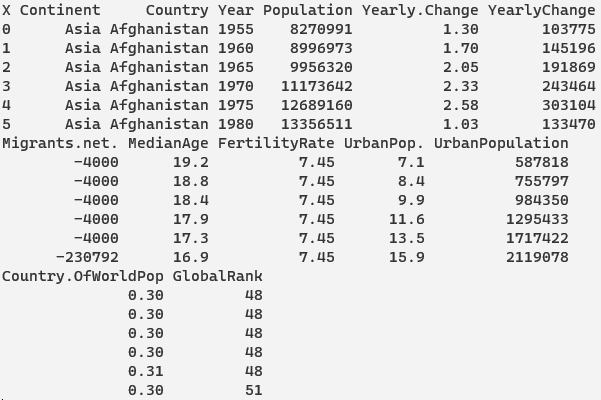
\includegraphics[width=.69\textwidth]{df.png}
	\end{figure}
\end{frame}

\begin{frame}
	\frametitle{The project}
	\begin{alertblock}{Goal}
		Study the growth of world population considering data from 1955 to 2020
	\end{alertblock}
	\begin{block}{Analysis}
		\begin{itemize}
			\item time-dependence of population growth in selected countries
			\item difference in population growth between different mainlands
			\item existence (in a country) of a relation between the yearly change of population and other observables
		\end{itemize}
	\end{block}
\end{frame}

\begin{frame}
	\frametitle{Population growth in the U.S.A.}
	\begin{figure}
		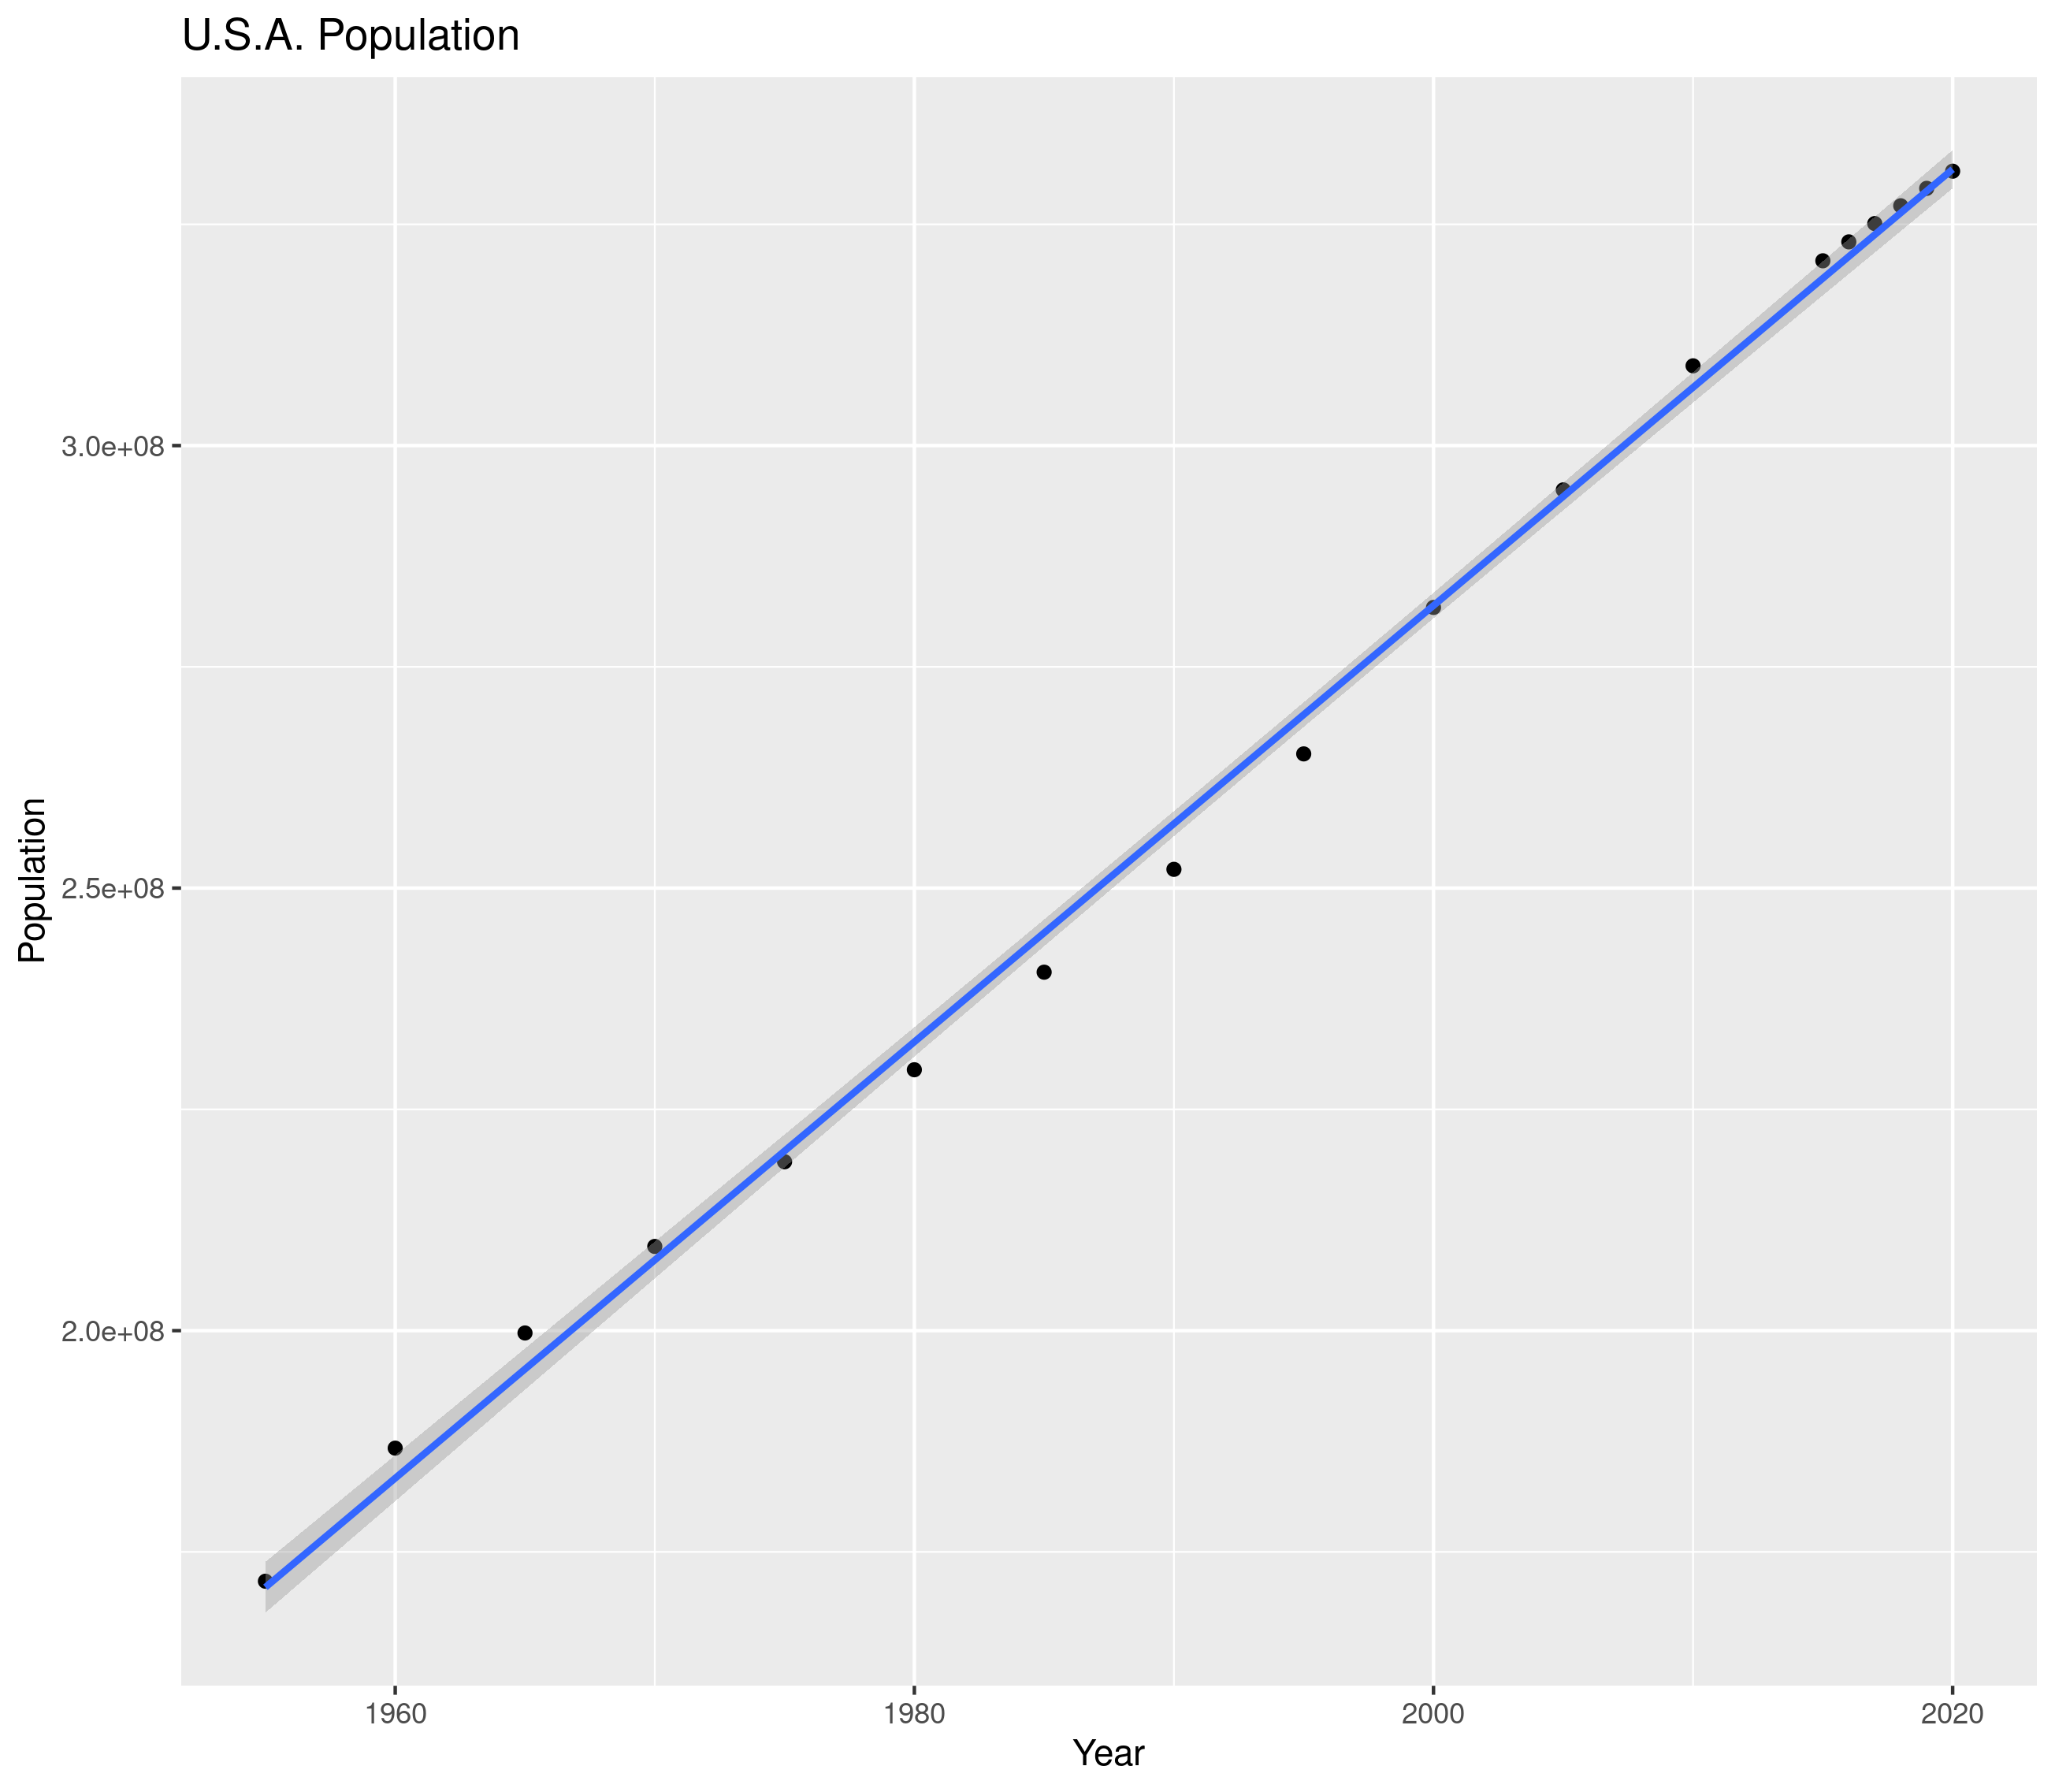
\includegraphics[width=.69\textwidth]{usa.png}
	\end{figure}
\end{frame}

\begin{frame}
	\frametitle{Population growth in the U.S.A.}
	\begin{exampleblock}{Fit results}
		\begin{itemize}
			\item $\text{slope} = \left(2.465 \pm 0.030\right) \times 10^6 \ ab/y$ \\
				$p_s < 2 \times 10^{-16}$
			\item $\text{intercept} = \left(-4.648 \pm 0.060\right) \times 10^9 \ ab$ \\
				$p_i < 2 \times 10^{-16}$
			\item $R^2 = 0.997$
		\end{itemize}
	\end{exampleblock}
	\begin{block}{Pearson's correlation test}
		\begin{itemize}
			\item $\text{p-value} < 2.2 \times 10^{-16}$
			\item $\rho = 0.999$
			\item C.I. $\left[0.997, 0.999\right]$ at $95\%$ C.L.
		\end{itemize}
	\end{block}
\end{frame}

\begin{frame}
	\frametitle{Population growth in Pakistan}
	\begin{figure}
		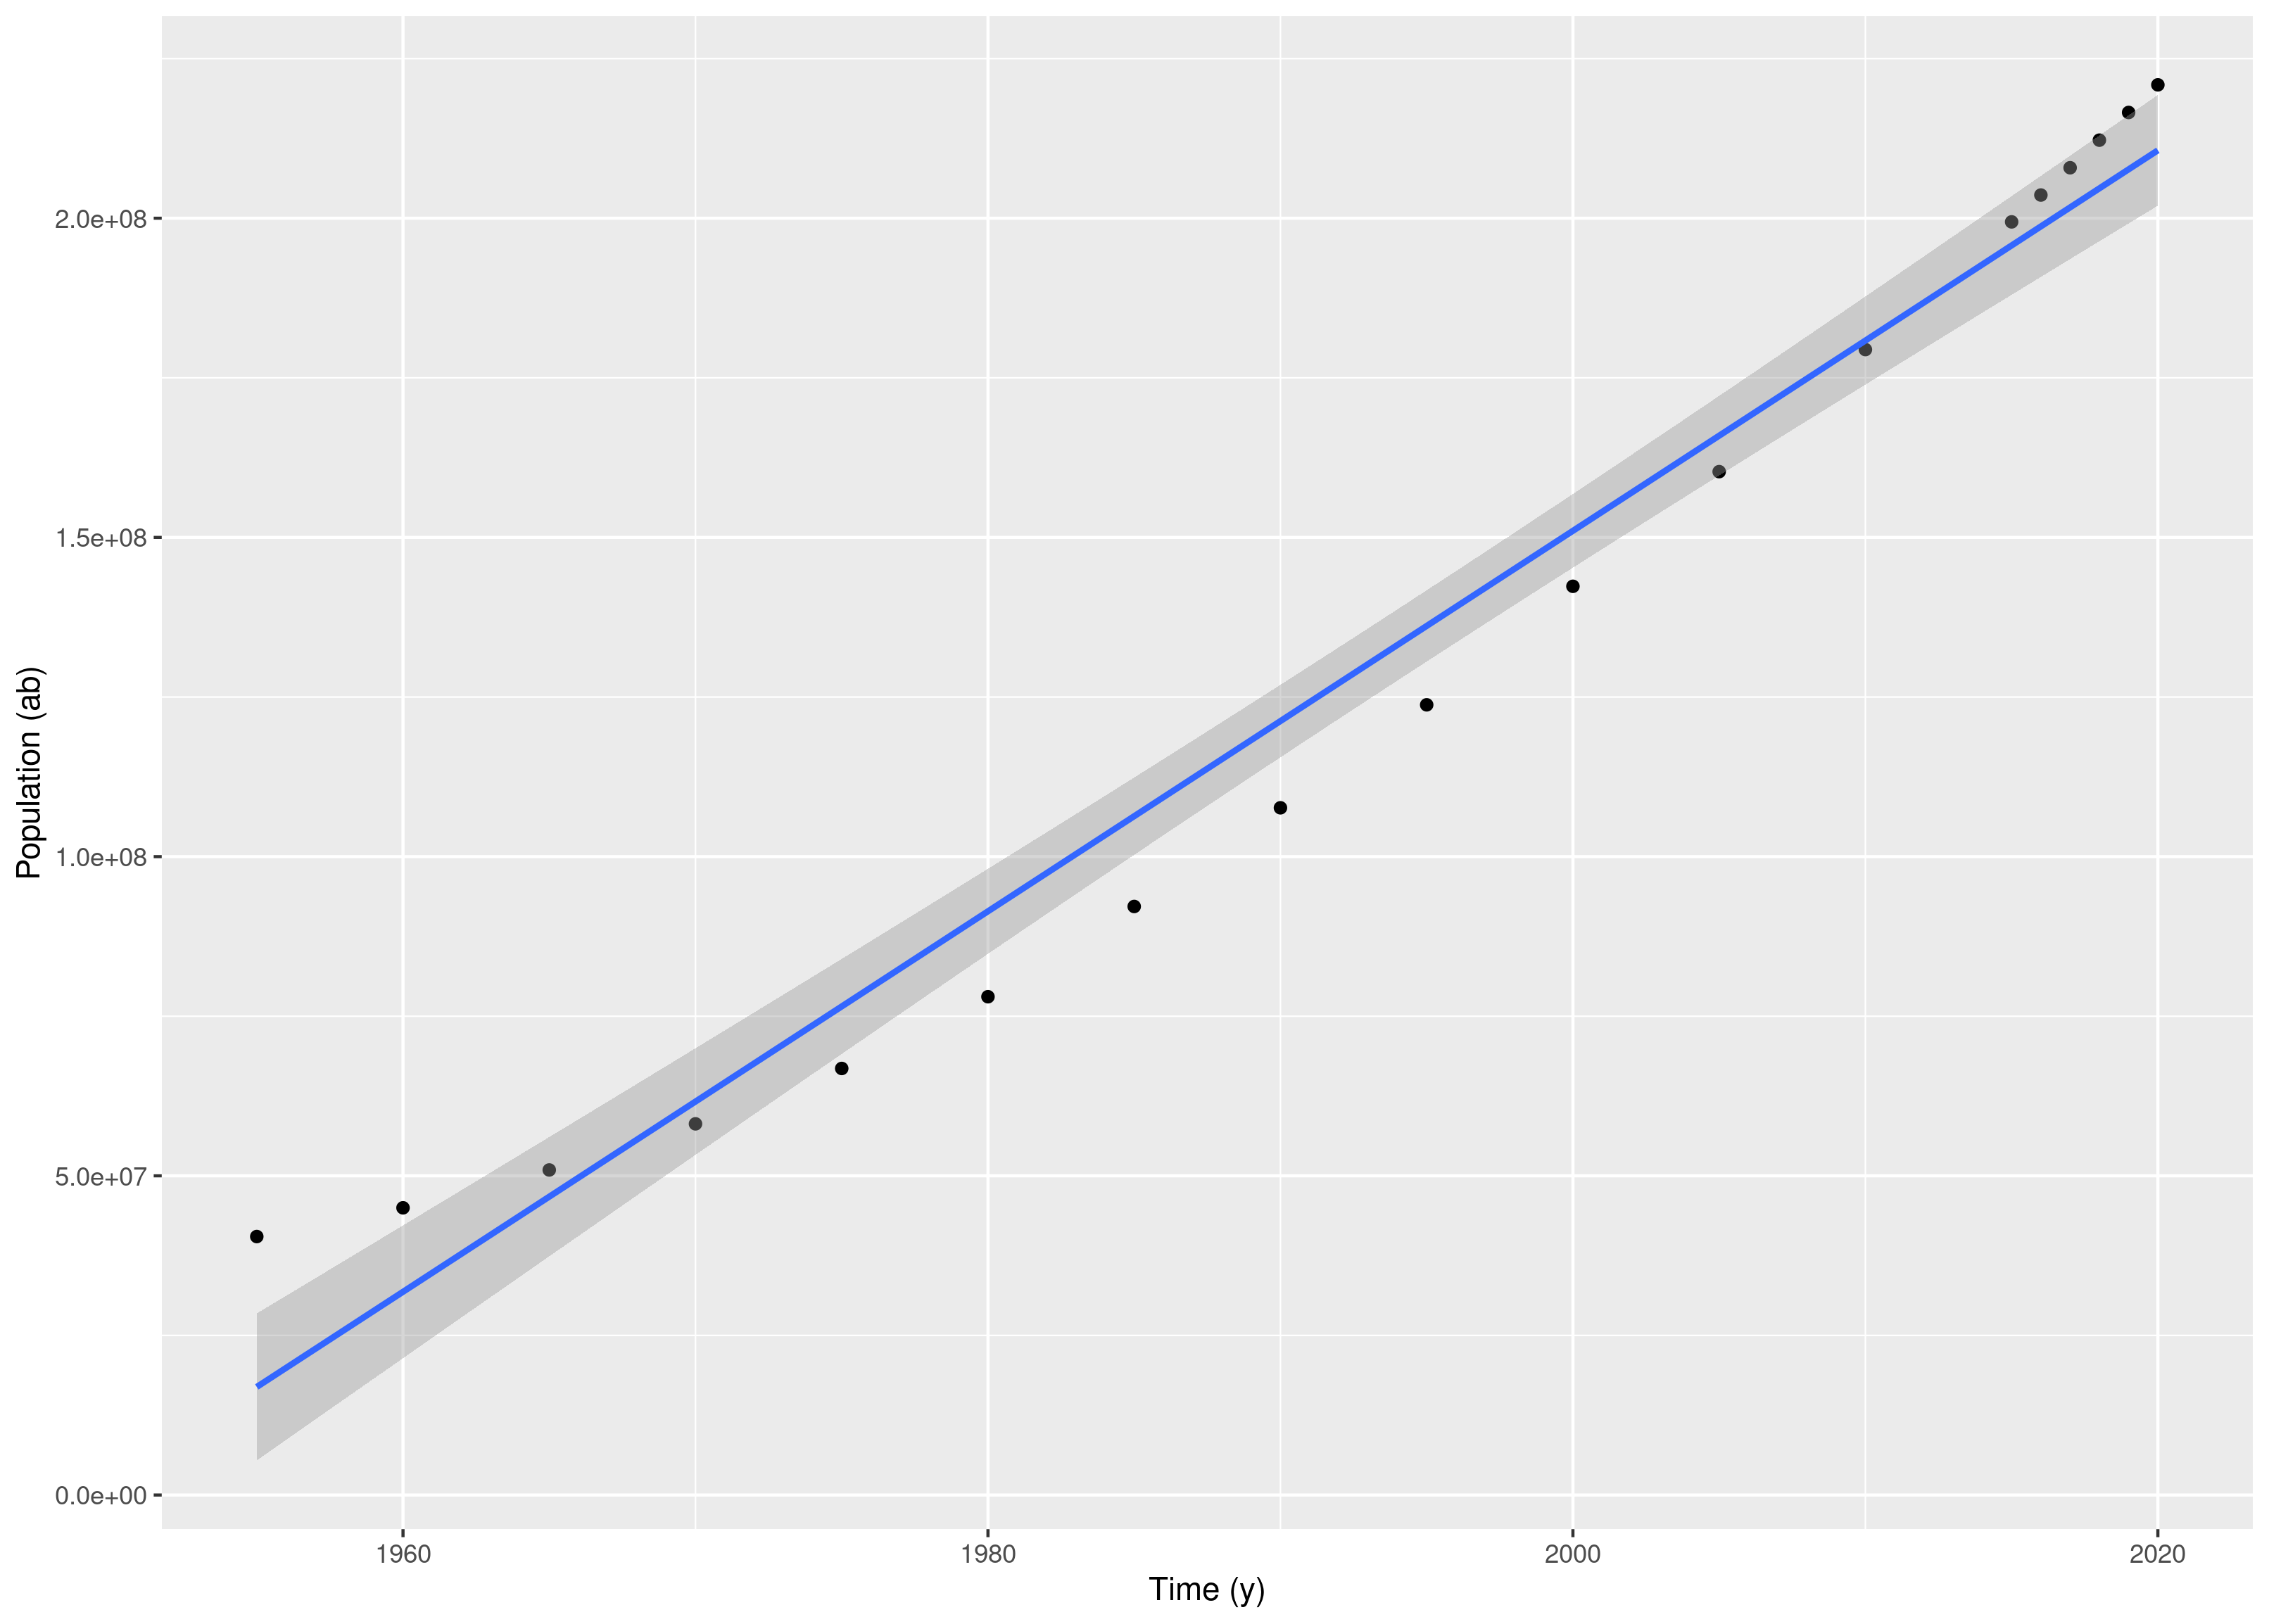
\includegraphics[width=.69\textwidth]{pak.png}
	\end{figure}
\end{frame}

\begin{frame}
	\frametitle{Population growth in Pakistan - log correction}
	\begin{figure}
		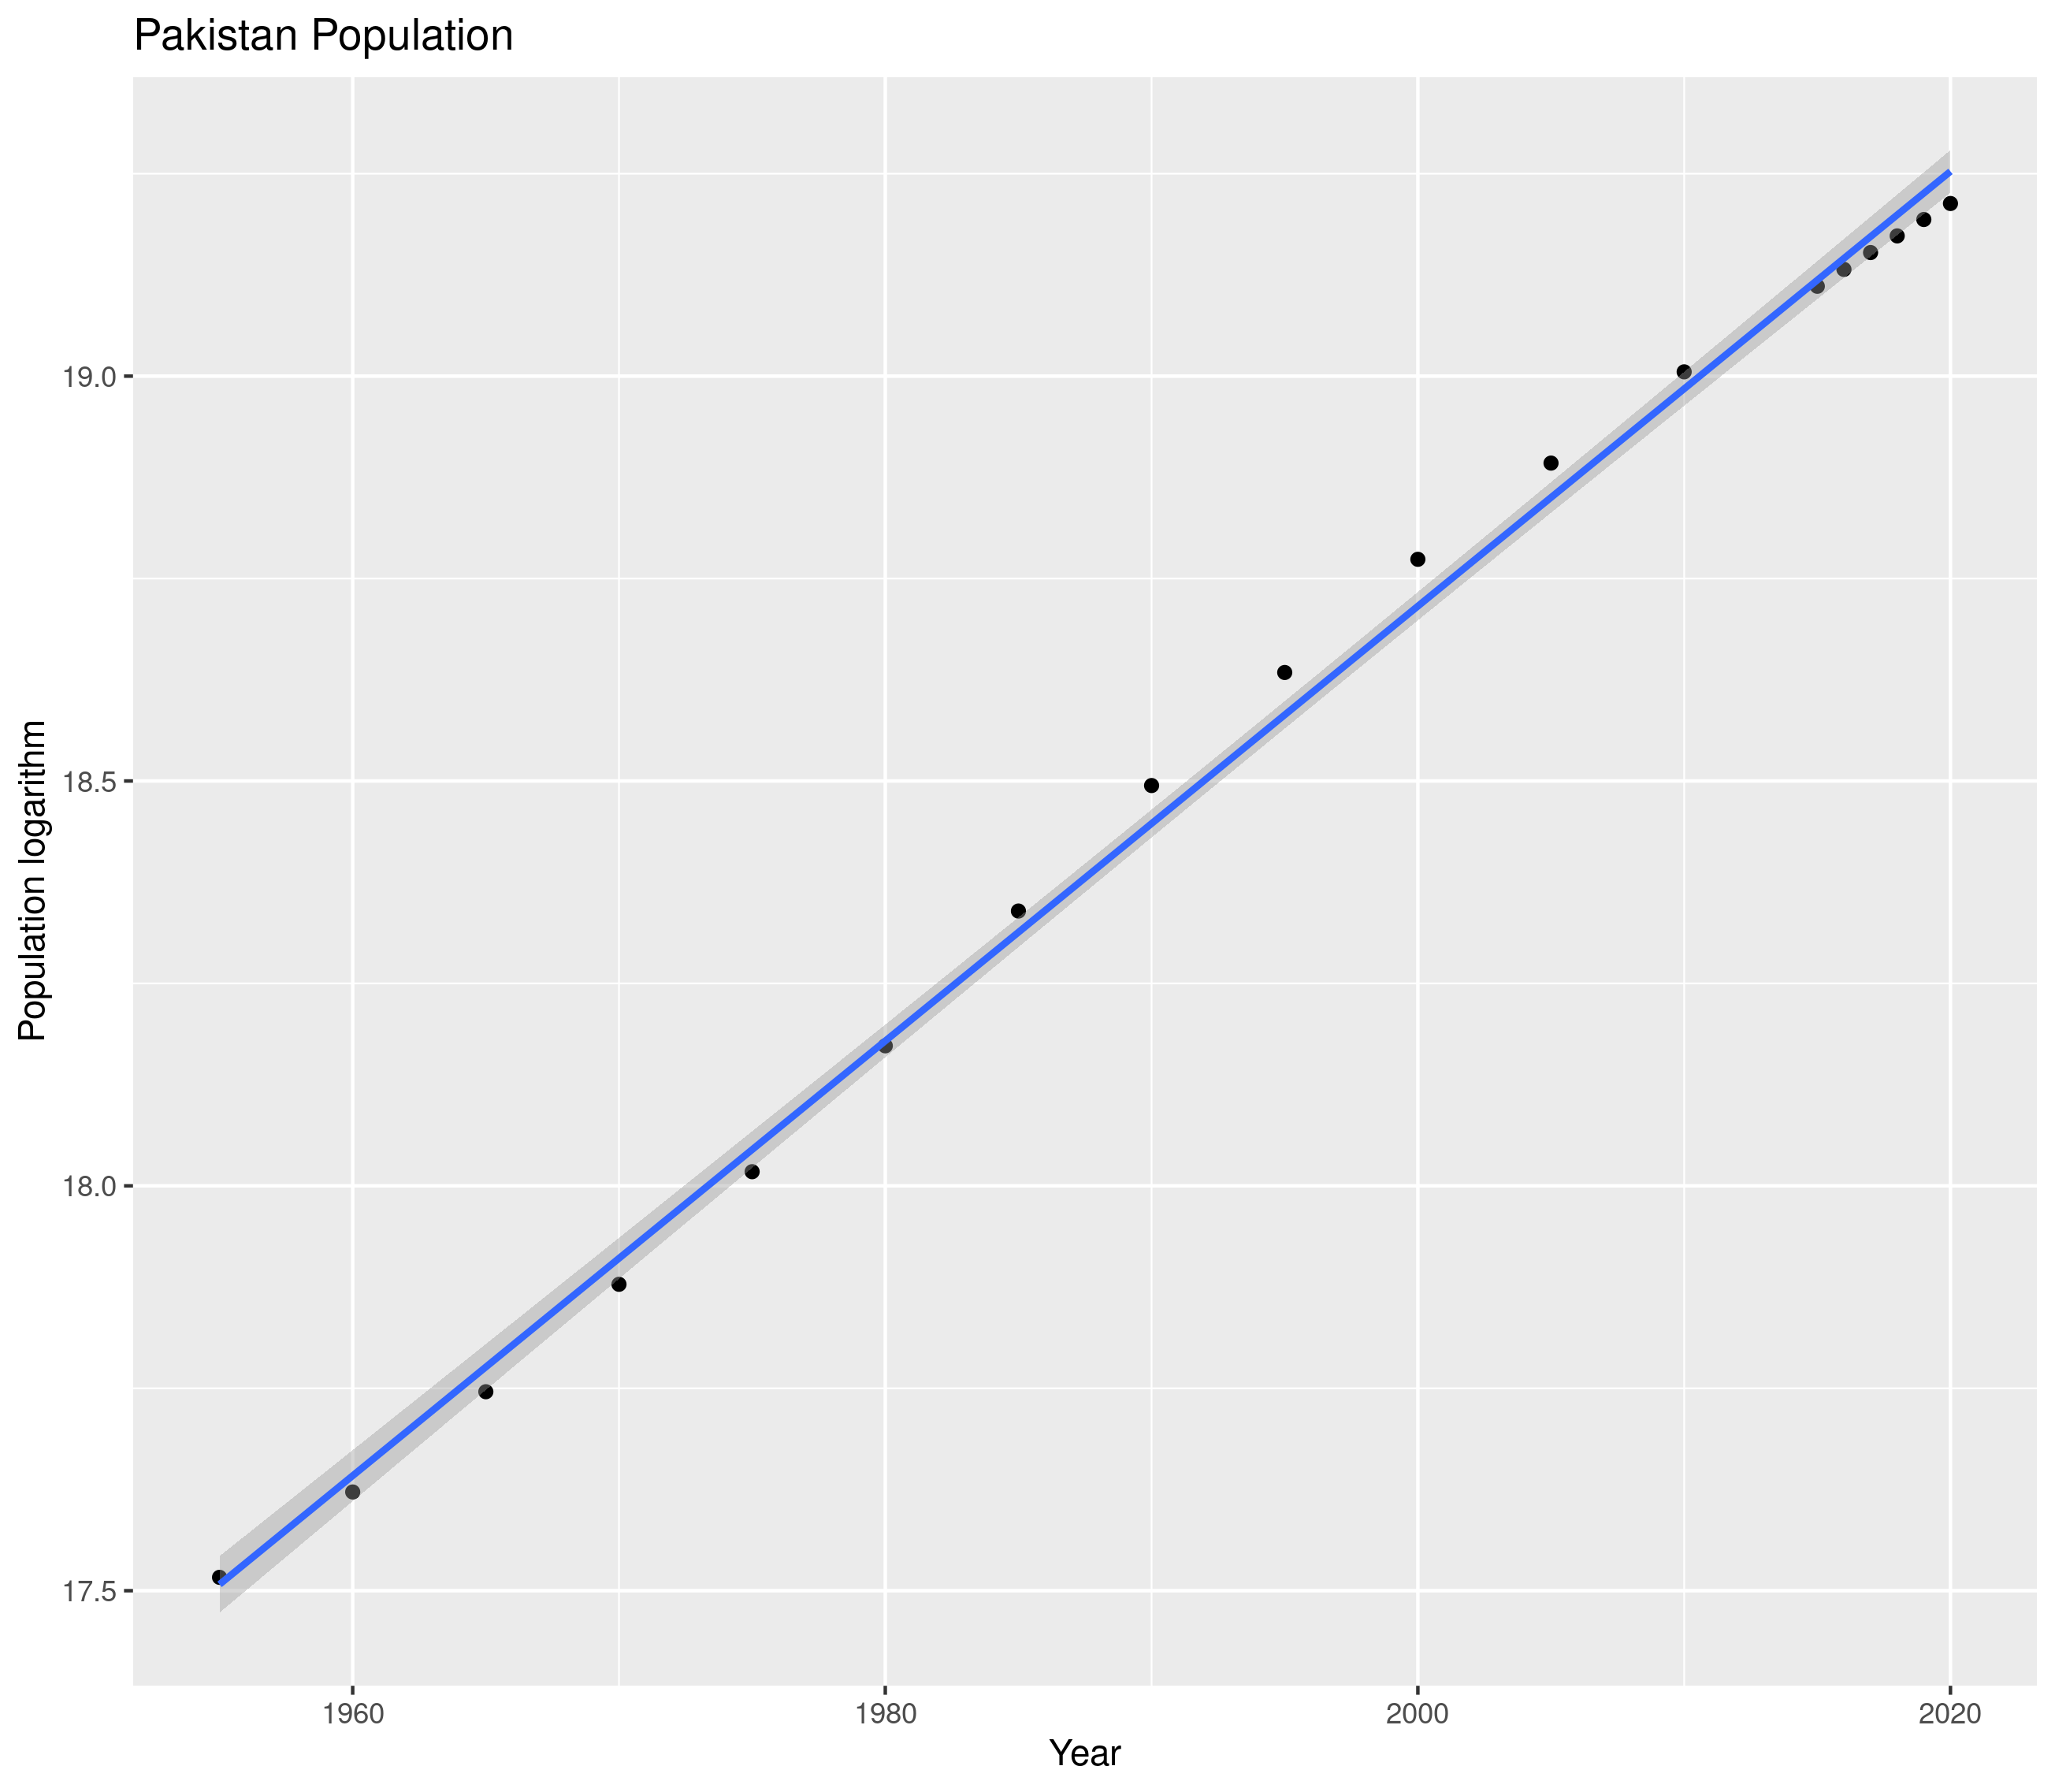
\includegraphics[width=.75\textwidth]{pak_log.png}
	\end{figure}
\end{frame}

\begin{frame}
	\frametitle{Population growth in Pakistan - log correction}
	\begin{exampleblock}{Fit results}
		\begin{itemize}
			\item $\text{slope} = \left(2.685 \pm 0.037\right) \times 10^{-2} \ ab/y$ \\
				$p_s < 2 \times 10^{-16}$
			\item $\text{intercept} = \left(-3.498 \pm 0.073\right) \times 10 \ ab$ \\
				$p_i < 2 \times 10^{-16}$
			\item $R^2 = 0.997$
		\end{itemize}
	\end{exampleblock}
	\begin{block}{Pearson's correlation test}
		\begin{itemize}
			\item $\text{p-value} < 2.2 \times 10^{-16}$
			\item $\rho = 0.998$
			\item C.I. $\left[0.996, 0.999\right]$ at $95\%$ C.L.
		\end{itemize}
	\end{block}
\end{frame}

\begin{frame}
	\frametitle{Hypothesis testing}
	Logarithm of population through time for Oceania (blue) and Asia (red).
	\begin{figure}
		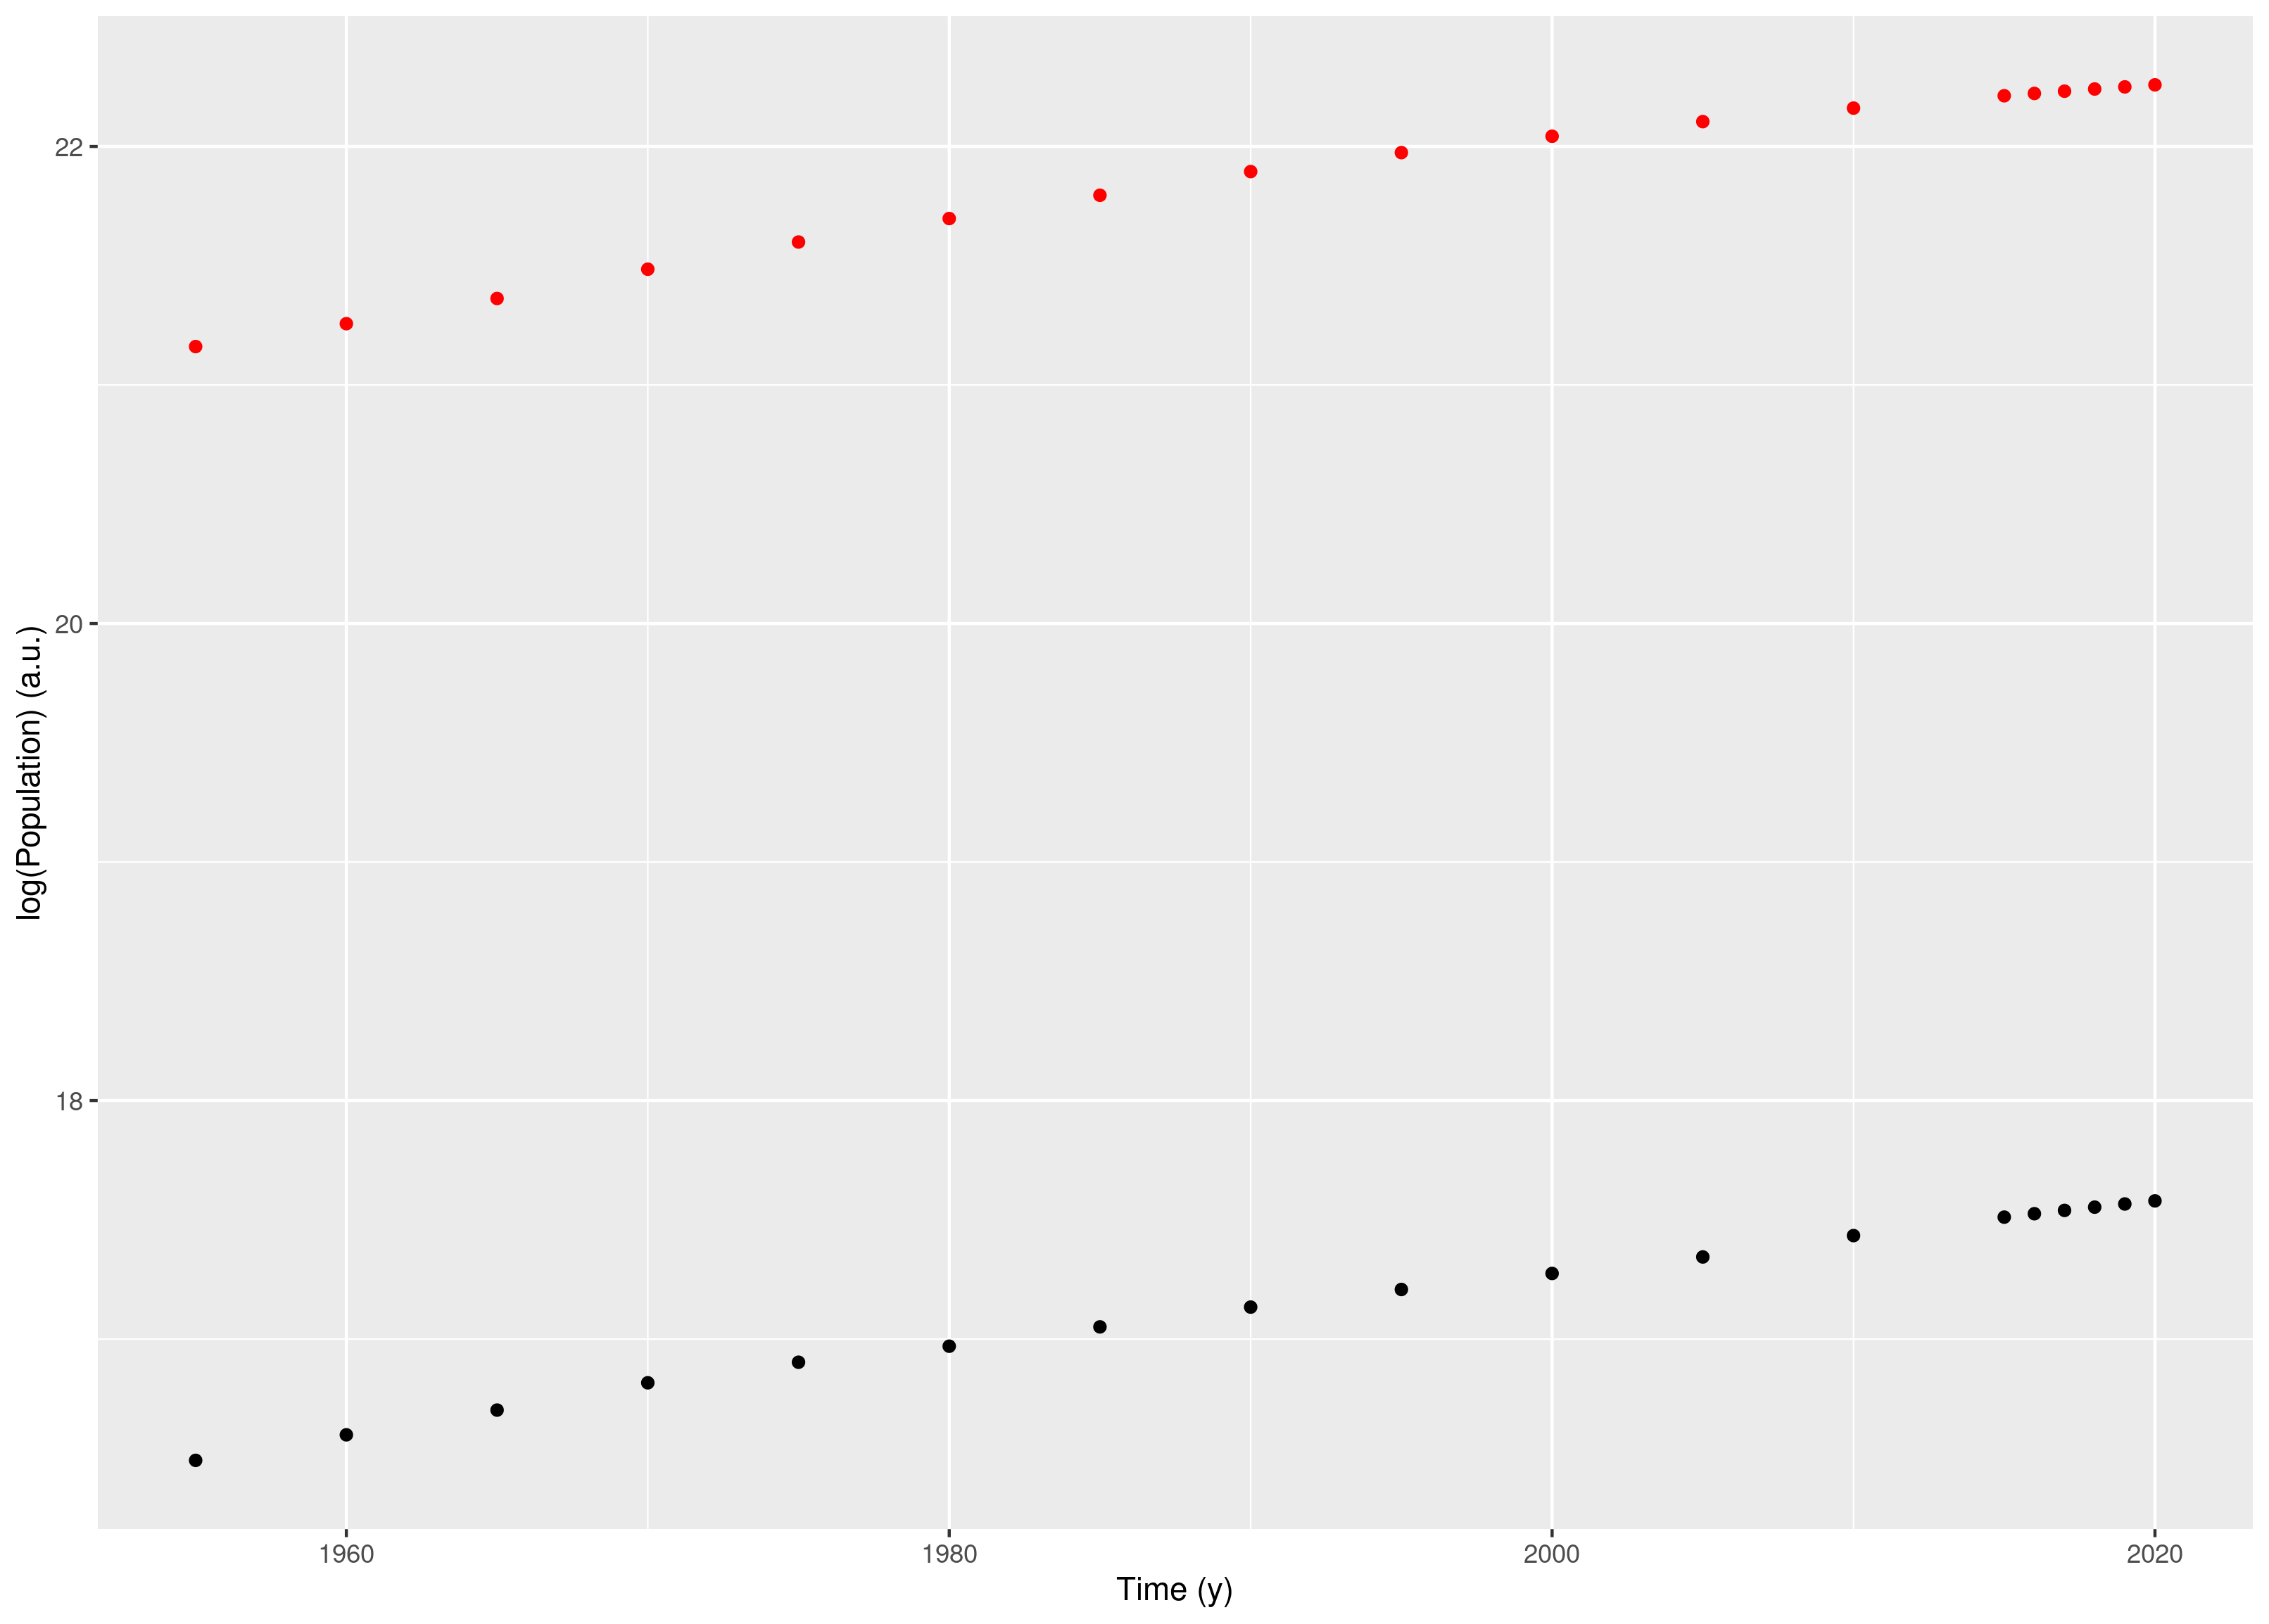
\includegraphics[width=.75\textwidth]{asia_oceania.png}
	\end{figure}
\end{frame}

\begin{frame}
	\frametitle{Hypothesis testing}
	Distribution of the logarithm of population for Oceania (blue) and Asia (red).
	\begin{figure}
		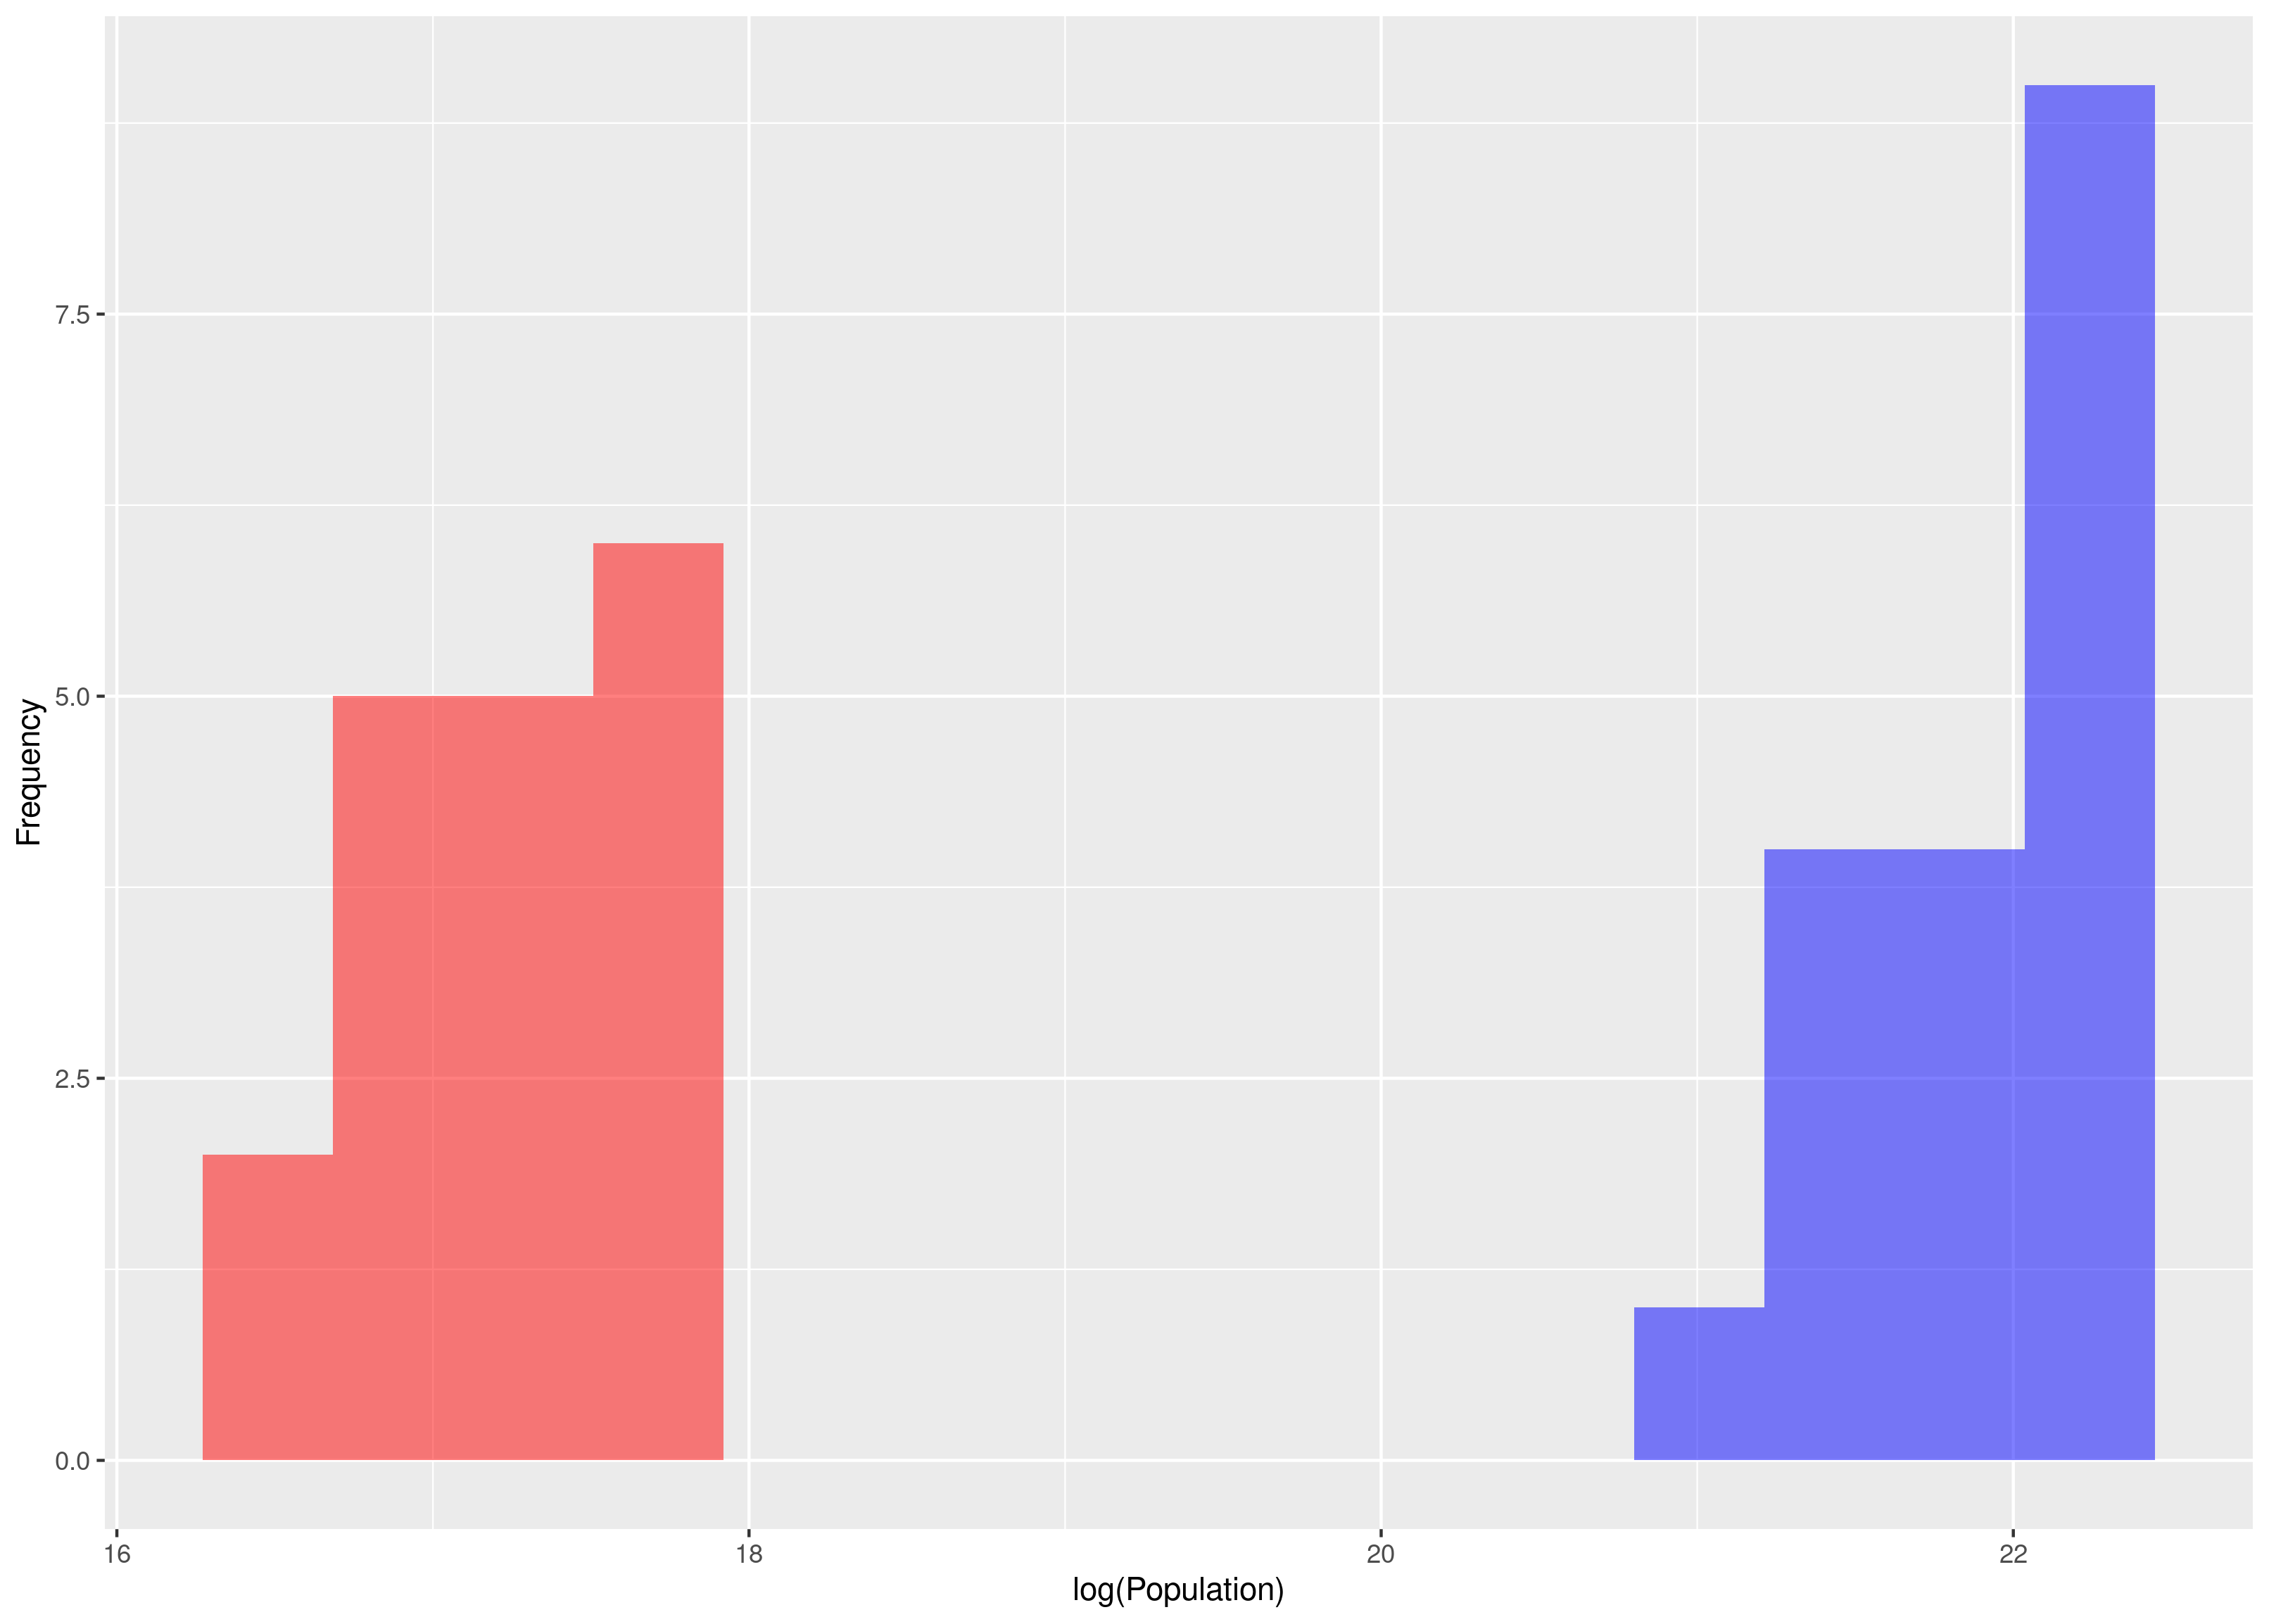
\includegraphics[width=.75\textwidth]{asia_oceania_hist.png}
	\end{figure}
\end{frame}

\begin{frame}
	\frametitle{Hypothesis testing}
	\begin{figure}
		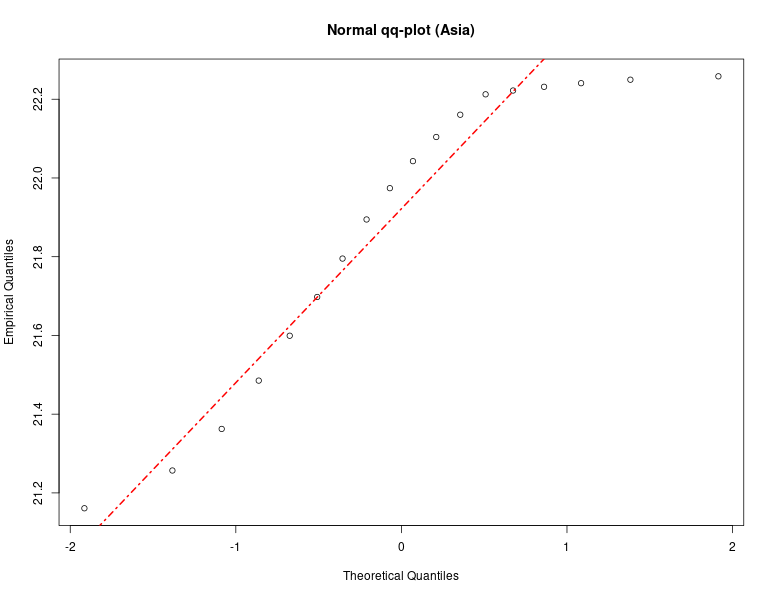
\includegraphics[width=.45\textwidth]{qqnorm_asia.png}
		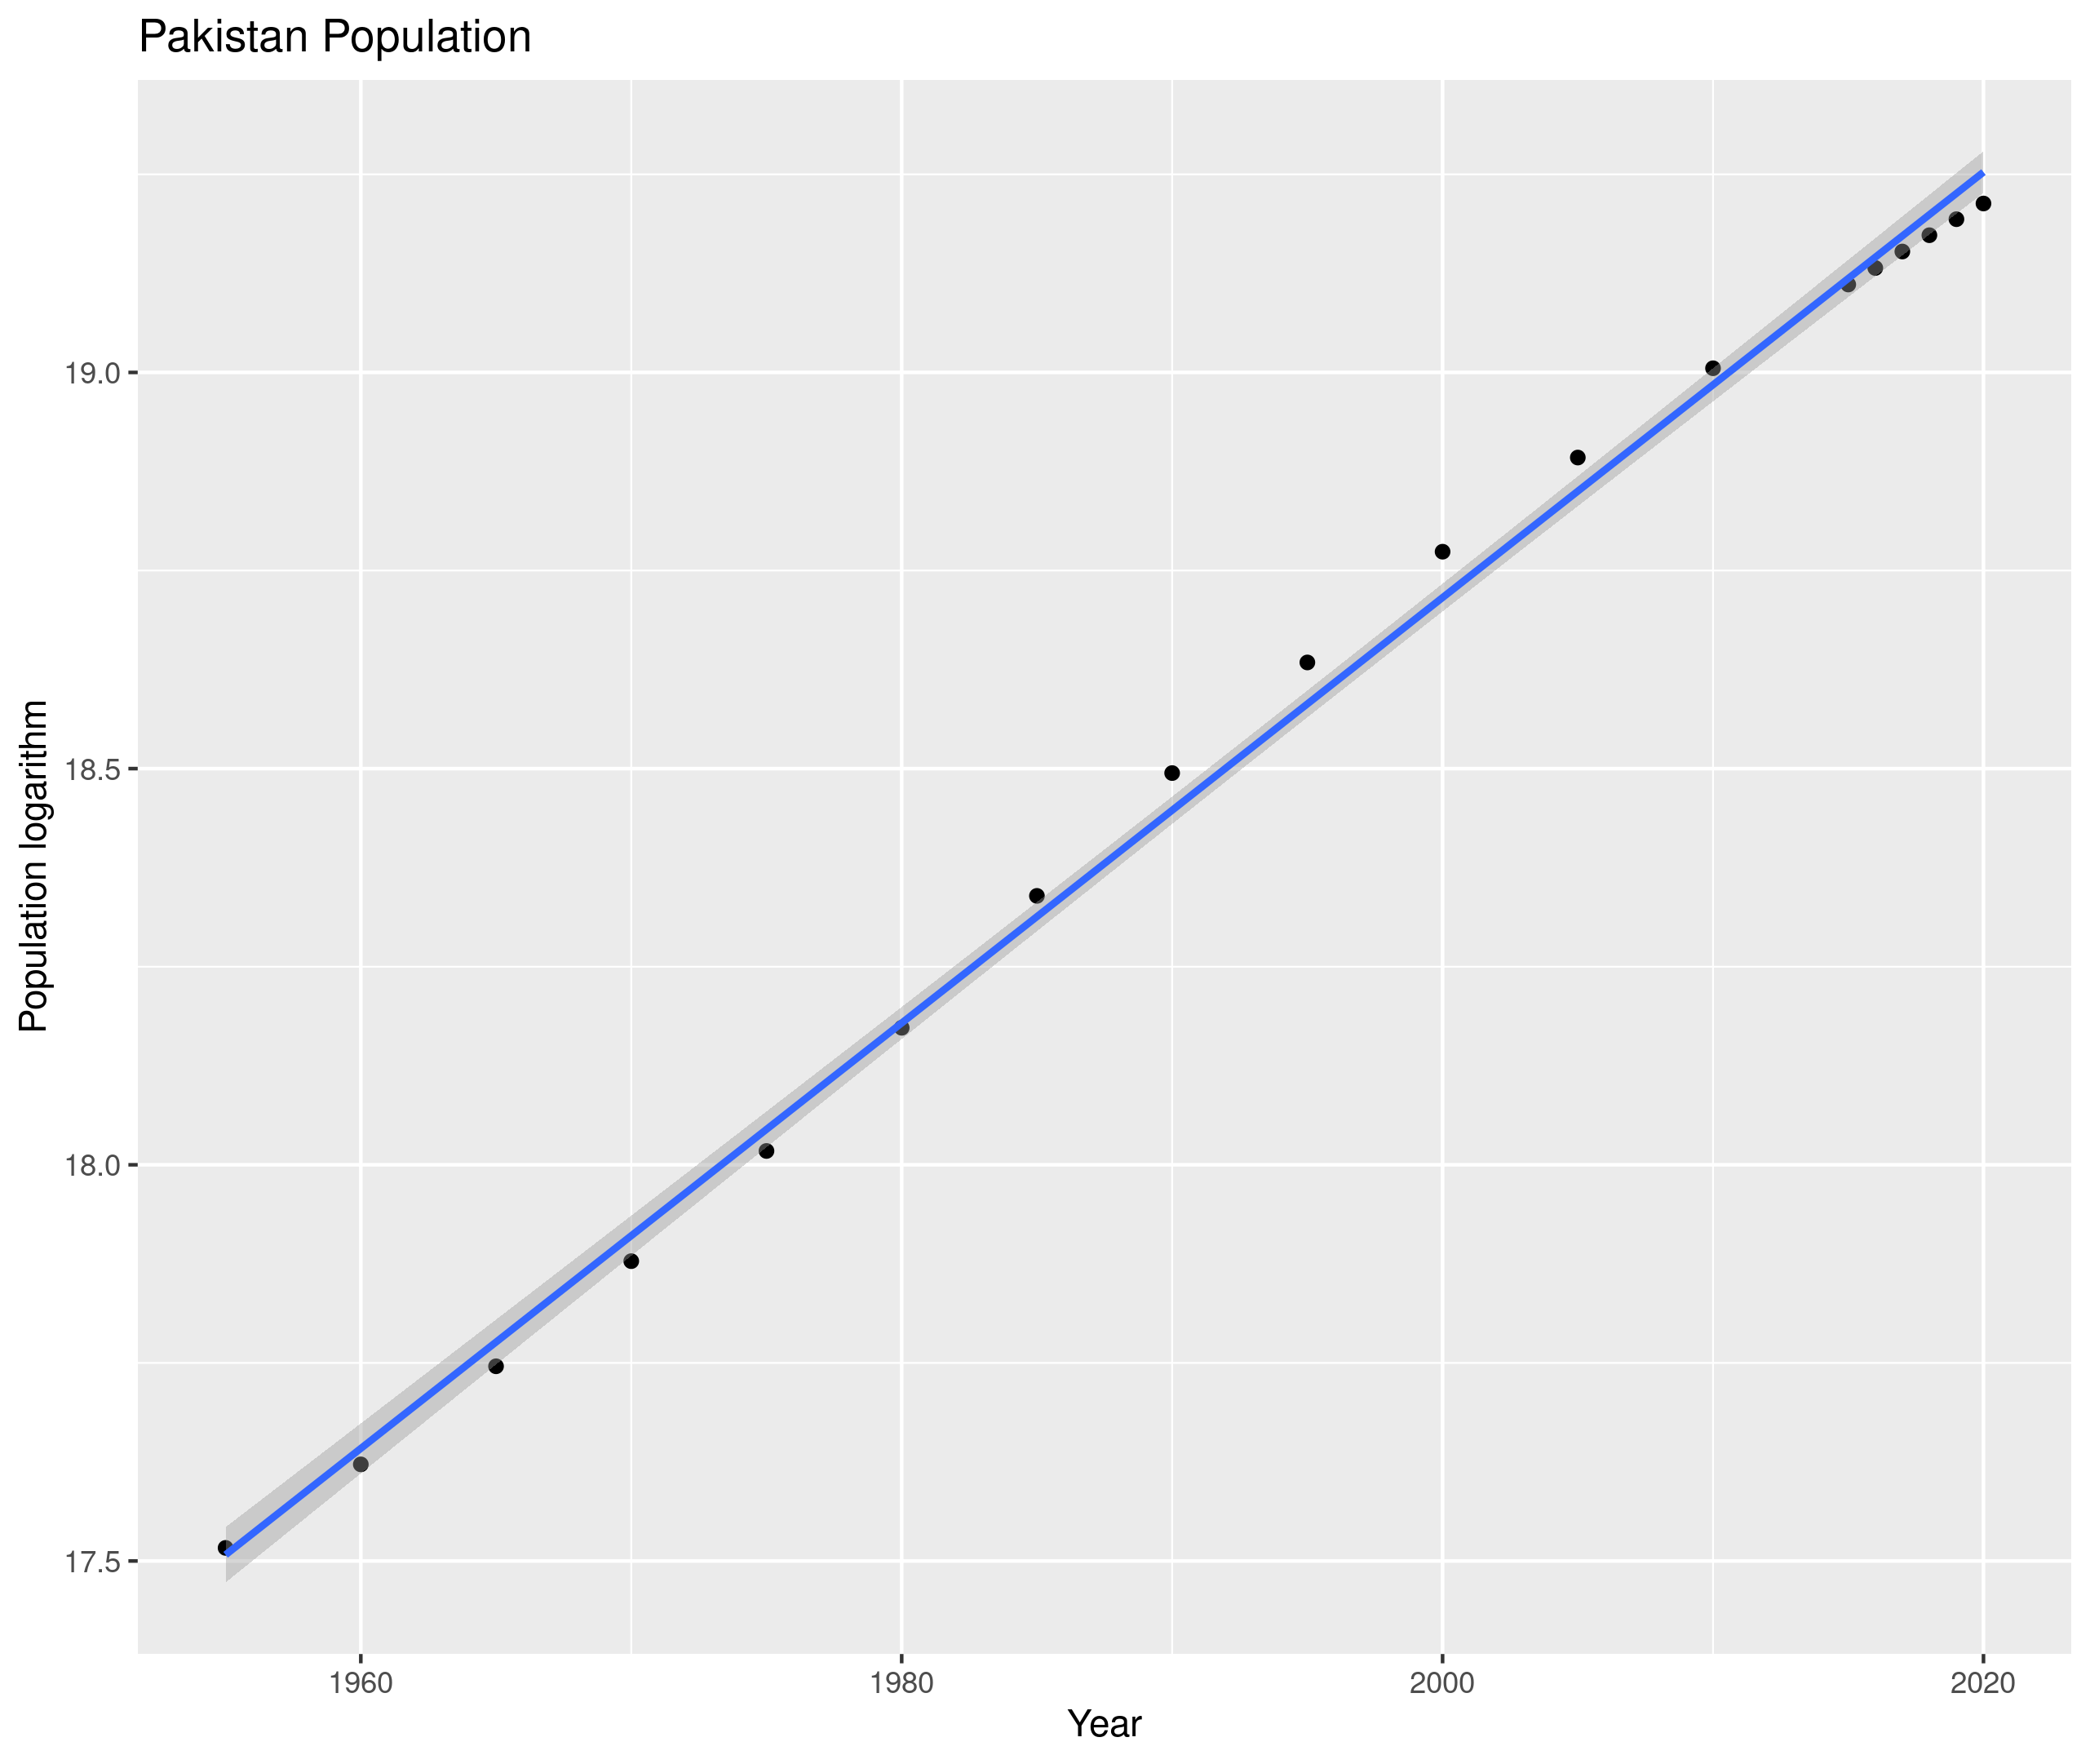
\includegraphics[width=.45\textwidth]{qqnorm_oceania.png}
	\end{figure}
	\begin{exampleblock}{Welch Two Sample t-test}
		\begin{itemize}
			\item $\mu_{asia} = 21.9 \ \left(\text{a.u.}\right)$
			\item $\mu_{oceania} = 17.2 \ \left(\text{a.u.}\right)$
			\item C.I. $\left[4.46, 4.96\right]$ at $95\%$ C.L.
			\item $\text{p-value} < 2.2 \times 10^{-16}$
		\end{itemize}
	\end{exampleblock}
\end{frame}

\begin{frame}
	\frametitle{Multilinear model}
	Let's see the yearly change of population (\%) in France with respect to all other variables
	\begin{figure}
		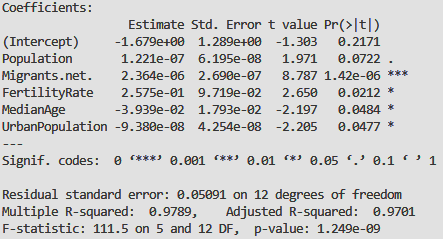
\includegraphics[width=.75\textwidth]{france.png}
	\end{figure}
\end{frame}

\begin{frame}[plain, noframenumbering] % The optional argument 'plain' hides the headline and footline
	\begin{center}
		{\Huge Thanks for the attention}
		
		\bigskip\bigskip % Vertical whitespace
		
		{\LARGE References:}
		
		\bigskip
		\small

		\url{https://www.kaggle.com/datasets/nguyenthicamlai/population-2022}

	\end{center}
\end{frame}

\begin{frame}[plain, noframenumbering]
	
\end{frame}

\begin{frame}[noframenumbering]
	\frametitle{USA analysis - residuals}
	\begin{figure}
		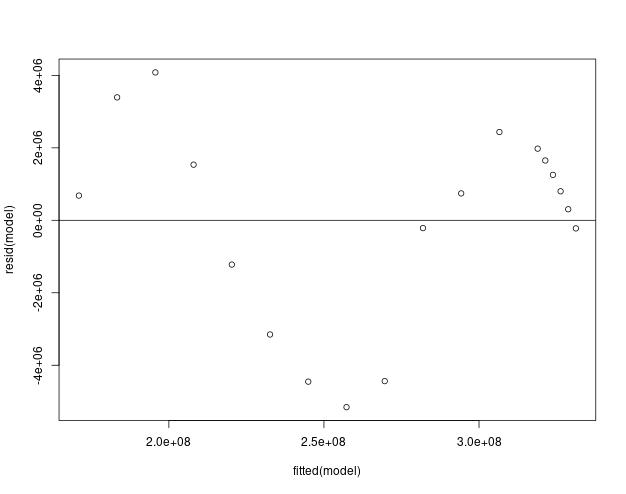
\includegraphics[width=.45\textwidth]{res_usa.png}
		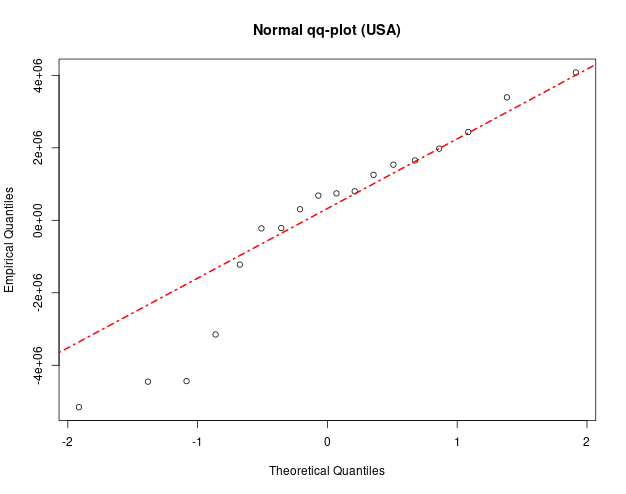
\includegraphics[width=.45\textwidth]{qq_usa.png}
	\end{figure}
\end{frame}
\begin{frame}[noframenumbering]
	\frametitle{Pakistan analysis - residuals}
	\begin{figure}
		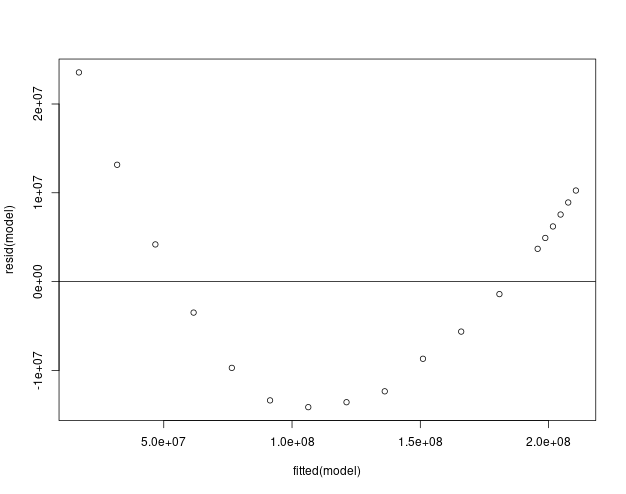
\includegraphics[width=.4\textwidth]{res_pak.png}
		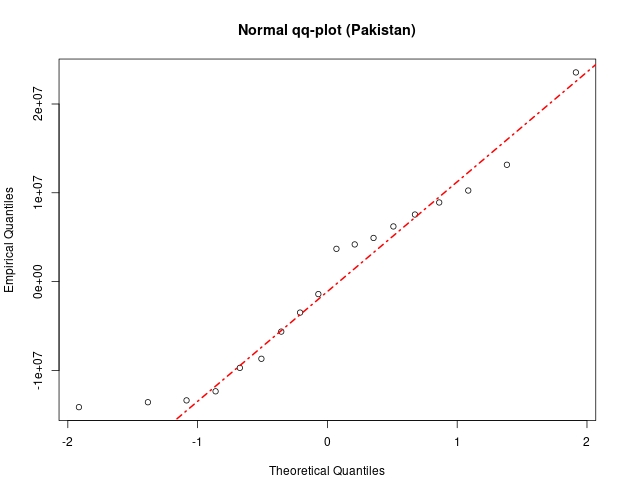
\includegraphics[width=.4\textwidth]{qq_pak.png}
	\end{figure}
	\begin{figure}
		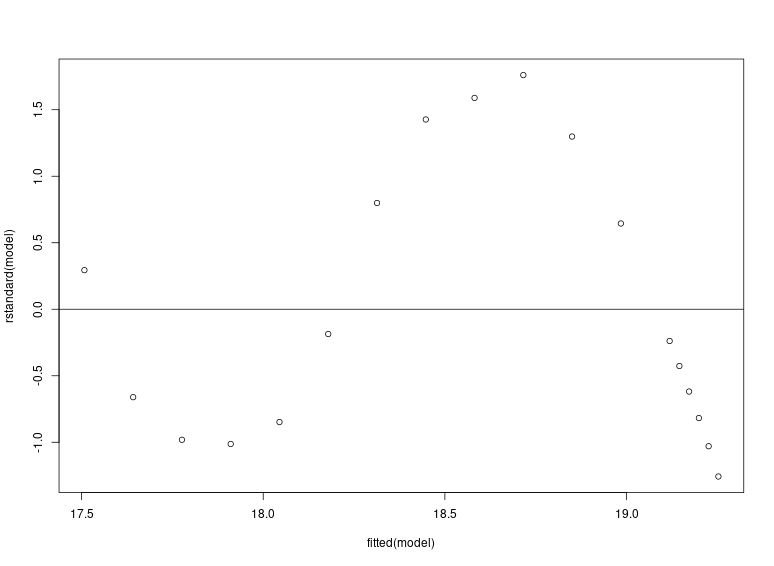
\includegraphics[width=.4\textwidth]{res_pak_log.png}
		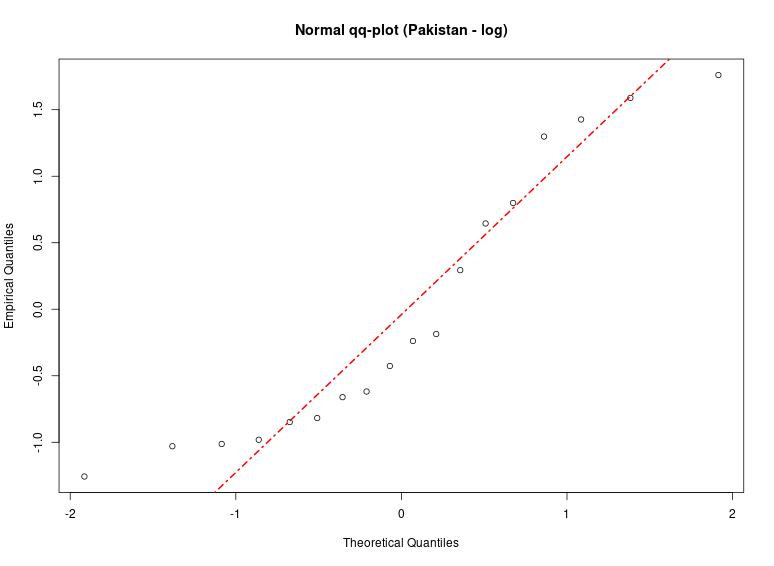
\includegraphics[width=.4\textwidth]{qq_pak_log.png}
	\end{figure}
\end{frame}

\end{document} 